\documentclass[11pt,a4paper]{article}
\usepackage[T1]{fontenc}
\usepackage[utf8]{inputenc}
\usepackage{newtxtext,newtxmath}
\usepackage{microtype}
\usepackage[a4paper,margin=1in]{geometry}
\usepackage{setspace,parskip}
\setlength{\parindent}{0pt}
\setlength{\parskip}{6pt plus 1pt minus 1pt}
\setstretch{1.15}
\usepackage[dvipsnames,svgnames]{xcolor}
\definecolor{accent}{HTML}{2B3A55}
\definecolor{accentlight}{HTML}{F4F5F7}
\usepackage{titlesec}
\titleformat{\section}{\normalfont\large\bfseries\scshape}{\thesection.}{0.6em}{}
\titleformat{\subsection}{\normalfont\normalsize\bfseries}{\thesubsection}{0.6em}{}
\titlespacing*{\section}{0pt}{18pt}{6pt}
\titlespacing*{\subsection}{0pt}{12pt}{3pt}
\usepackage{fancyhdr}
\pagestyle{fancy}\fancyhf{}
\renewcommand{\headrulewidth}{0pt}
\fancyhead[C]{\small\itshape\color{gray} Financial Fraud Detection Using ANN with Imbalanced Learning}
\fancyfoot[C]{\small\color{gray}\thepage}
\setlength{\headheight}{14pt}
\usepackage{booktabs,array,graphicx}
\usepackage[colorlinks=true,linkcolor=accent,urlcolor=accent,citecolor=accent]{hyperref}
\emergencystretch=2em
\begin{document}
\begin{center}
{\bfseries\LARGE Financial Fraud Detection Using Artificial Neural Networks with Imbalanced Learning}\\[8pt]
{\large Reproducible IEEE-CIS Experimental Study}\\[4pt]
{\normalsize\itshape Research prototype report}
\end{center}
\vspace{8pt}
\begin{abstract}
Financial fraud detection combines rare positive events, changing transaction behaviour, and costly classification errors. This study compares three configurable feed-forward artificial neural networks (ANNs): an unweighted baseline, categorical-aware synthetic oversampling, and class-weighted binary cross-entropy. IEEE-CIS transaction and identity records are joined with validated unique keys. A shared chronological train--validation--test protocol preserves natural holdout prevalence, fits preprocessing on training only, and selects checkpoints and thresholds on validation data. Three initialization seeds are evaluated for each method on full labeled data, with a separate development-sample study. A PyTorch worker, FastAPI service, notebook, and Next.js laboratory share canonical artifacts containing configurations, splits, probabilities, metrics, and software versions. Generated results emphasize average precision, precision, recall, and missed fraud. The system supports auditable research and model inspection; local validation does not establish suitability for production financial decisions.
\end{abstract}
\noindent\textbf{Keywords:} financial fraud; artificial neural network; imbalanced learning; SMOTENC; cost-sensitive classification; temporal evaluation.

\section{Introduction}
Fraud detectors return scores, while operational decisions depend on thresholds. A narrow alert set can achieve high precision but miss fraud; a broader set can increase recall and legitimate-transaction reviews. Ranking quality and decision-rule performance therefore require separate evaluation.

An unweighted ANN receives many more legitimate than fraudulent observations. Good average loss or accuracy can conceal minority-class failure. Resampling changes the training distribution, whereas class weighting changes contributions to the objective. Neither guarantees better ranking, calibrated probabilities, or acceptable workload. Evaluation must retain the original class prevalence.

Recent reviews identify imbalance, changing fraud patterns, and deployment constraints \cite{btoush2023review,strelcenia2023survey}. Empirical augmentation studies motivate ANN comparisons \cite{cheah2023smotegan}, while leakage analyses warn that faulty preprocessing can inflate apparent performance \cite{hayat2025leakage}. This project consequently treats the protocol as part of the result.

The contribution is a reproducible comparison and interactive research system, not a novel neural architecture. Training changes create immutable runs; threshold changes reuse saved probabilities. Notebook, dashboard, and paper read identical artifacts. Synthetic fixtures validate software only, and development samples remain distinct from full-data evidence.

\section{Literature Survey}
Btoush et al.'s 2023 systematic review organizes machine/deep learning fraud detection and identifies practical challenges \cite{btoush2023review}. Its survey coverage ends before publication; it motivates this study but does not establish an optimal IEEE-CIS model.

Strelcenia and Prakoonwit review GAN augmentation, including instability and synthetic-sample quality \cite{strelcenia2023survey}. These concerns support cautious interpretation of generated minority transactions. Transparent categorical-aware oversampling offers a narrower experimental intervention.

Cheah et al. compare SMOTE, GAN, and hybrid augmentation with neural classifiers on the European cardholder benchmark \cite{cheah2023smotegan}. This is a close ANN/imbalance precedent, but a different dataset. Their description of scaling before splitting raises a potential leakage concern inferred from the stated order, not independently replicated here.

Hayat and Magnier deliberately compare faulty and corrected evaluation procedures \cite{hayat2025leakage}. Their empirical methodological study directly supports training-only resampling, separate selection data, and untouched holdouts.

Darwish et al. describe sampling and multistage classification including IEEE-CIS evaluation \cite{darwish2025abc}. Different models and insufficiently matching split information prevent direct ranking against this project.

Habibpour et al. propose dropout/ensemble uncertainty methods for deep fraud detection and identify IEEE-CIS \cite{habibpour2023uncertainty}. The journal metadata is verified, but closed full text limits exact protocol verification. Preprint experimental numbers and its different author list are not transferred to the journal citation.

\section{Problem Statement}
For transaction attributes $x$ and label $y\in\{0,1\}$, learn $p_\theta(x)$ and flag when $p_\theta(x)\geq\tau$. Compare three ANN learning strategies under identical observations and preprocessing. Report ranking, fraud capture, alert quality, errors, resource use, and reproducible evidence rather than a single accuracy value.

\section{Dataset Description}
The supplied IEEE-CIS archive contains 590,540 training transactions (394 columns), 144,233 identity records (41 columns), and separate unlabeled competition-test files \cite{kaggleieee}. CRC checks, file hashes, schemas, binary targets, and unique nonmissing keys are verified. A one-to-one validated left join preserves transaction rows, yielding 434 joined columns.

\texttt{TransactionID} is a join key, and \texttt{isFraud} is the target; neither is a predictor. \texttt{TransactionDT} is relative elapsed time, not a calendar timestamp. Missing identity attributes remain available for training-fitted imputation. Unlabeled competition test data never supplies evaluation labels. A documented 57-predictor subset limits dense encoding costs.

\section{Methodology}
\subsection{Shared Split and Preprocessing}
Before splitting, exact covariate duplicates are removed without using labels, identifiers, or relative time. This conservative procedure prevents identical full predictor records crossing partitions but does not guarantee entity or near-duplicate isolation.

Rows are chronologically ordered with deterministic identifier tie-breaking. Approximately 70/15/15 proportions define training, validation, and test; equal relative times stay together. Split identifiers and hashes are retained. Development sampling uses a separate fixed split seed, so changing model initialization does not change held-out observations. Random stratification is optional and has different temporal assumptions.

Numerical imputation and standard/robust scaling fit training only. Categorical imputation and ordinal/one-hot encoders also fit training only. Known integer-coded categories retain categorical treatment. Ordinal codes are used within SMOTENC, followed by one-hot encoding for the ANN. Unknown categories are reported at inference; exact input schemas reject arbitrary fields. Optional zero-variance removal is unsupervised and training-fitted.

\subsection{Three ANN Learning Strategies}
The ANN uses configurable hidden layers, activation, dropout, batch normalization, optimizer, learning rate, and regularization, ending in one logit. Sigmoid scores support inference, while numerically stable BCE operates on logits:
\begin{equation}
\mathcal L=-\frac1n\sum_i\left[w_1y_i\log p_i+w_0(1-y_i)\log(1-p_i)\right].
\end{equation}
The baseline sets $w_0=w_1=1$. L1 is explicit; the L2 setting is optimizer weight decay, decoupled for AdamW. Adam, AdamW, and SGD are supported.

The oversampling ANN retains unweighted loss. Numeric-only inputs permit SMOTE \cite{chawla2002smote}; mixed inputs use SMOTENC, whose categorical choices avoid interpolating arbitrary category codes. Category-only automatic mode uses explicitly reported random oversampling. Ratio and neighbor count are configurable; original/resampled counts are recorded. Resampling changes training only. High-dimensional distances and implausible synthetic combinations remain limitations.

The cost-sensitive ANN applies positive configurable $w_1$ and $w_0$ without oversampling. Larger fraud weights are not automatically better. Training weights and the probability cutoff are distinct quantities.

\subsection{Validation-Based Selection}
Checkpoint selection and early stopping use a configurable validation criterion, AP by default. A fixed 99-point validation threshold grid optimizes the selected measure, F1 in these runs. The selected model then produces final-test probabilities. Test labels never select checkpoints, stopping, or thresholds. Dashboard test-threshold inspection is explicitly post-hoc.

\section{Experimental Setup}
The Windows environment has an Intel Core i7-12700H, 20 logical processors, and approximately 16 GB RAM. Although a 4 GB RTX 3050 Ti is detected, executed runs use CPU PyTorch, with four computation threads and deterministic algorithms. Python 3.12, pinned dependencies, and an installed-package lock document the environment.

Seeds 42, 43, and 44 are evaluated on both full data and a separate deterministic 30,000-row development sample. Features, architecture, split, and training budget are held fixed across the three methods. Seed variation measures optimization/resampling variability on one window, not independent temporal generalization.

\begin{table}[ht]
\centering\small
\caption{Recorded primary configuration.}
\begin{tabular}{ll}
\toprule Parameter & Value \\
\midrule
Hidden layers & [64, 32] \\
Activation / dropout & relu / [0.2, 0.1] \\
Batch normalization & False \\
Optimizer / learning rate & adam / 0.001 \\
Epoch limit / patience & 15 / 5 \\
Batch size & 256 \\
L1 / weight decay & 0.0 / 0.0001 \\
Class weights (weighted only) & 1.0 / 20.0 \\
Oversampling ratio / neighbors & 0.3 / 5 \\
Split seed & 2026 \\
Numerical processing & median / standard \\
Original feature subset & 57 predictors \\
\bottomrule
\end{tabular}
\end{table}

AP summarizes the precision--recall staircase, $\mathrm{AP}=\sum_k(R_k-R_{k-1})P_k$, rather than trapezoidal integration of compressed plot points. Probability-based ROC-AUC accompanies accuracy, precision, recall, F1, specificity, error rates, balanced accuracy, Matthews correlation, and all confusion counts. AP and missed fraud remain prominent because high accuracy can conceal failed minority detection.

Fifty IID bootstrap resamples yield descriptive percentile intervals for AP and ROC-AUC, with valid replicate counts retained. They do not account for temporal/entity dependence. Training timing excludes preprocessing/resampling; total pipeline timing includes them. Test inference timing uses transformed features and excludes HTTP latency.

The independent worker atomically claims SQLite WAL jobs and records progress/heartbeats, cancellation, failure, and completion. HTTP requests submit validated jobs instead of running lengthy training. Immutable artifacts store configurations/hashes, dataset fingerprints, split IDs, schemas, weights, fitted preprocessors, histories, thresholds, probabilities, timings, and versions. Tests cover leakage invariants, metrics, save/load, schema validation, concurrent claims, cancellation, API errors, and frontend updates.

\section{Experimental Results}
IEEE-CIS full labeled data, 590,053 observations; 88,508 fixed test observations. Separate initialization seeds share one split.

\begin{table}[ht]
\centering\small
\caption{Full-data comparison at validation-selected cutoffs: mean $\pm$ sample standard deviation across initialization seeds.}
\begin{tabular}{lrrrr}
\hline Method & AP & Precision & Recall & F1 \\
\hline
Baseline ANN & 0.387 $\pm$ 0.009 & 0.451 $\pm$ 0.006 & 0.379 $\pm$ 0.011 & 0.411 $\pm$ 0.004 \\
SMOTENC + ANN & 0.427 $\pm$ 0.007 & 0.485 $\pm$ 0.054 & 0.423 $\pm$ 0.029 & 0.450 $\pm$ 0.008 \\
Weighted ANN & 0.375 $\pm$ 0.011 & 0.430 $\pm$ 0.059 & 0.381 $\pm$ 0.006 & 0.403 $\pm$ 0.030 \\
\hline
\end{tabular}
\end{table}

The test fraud prevalence is 3.488\%. The completed group contains 9 runs on a common fingerprint and split hash. SMOTENC + ANN has the highest recorded AP in this group; this internal descriptive result does not establish general superiority.

Baseline ANN records mean AP 0.3870. For the first seed, precision is 0.4437, recall is 0.3907, and F1 is 0.4155 at validation-selected cutoff 0.13. It flags 2,718 of 88,508 test transactions, including 1,512 false positives, while missing 1,881 frauds.

The IID test AP interval is [0.3820, 0.4163] from 50 valid bootstrap replicates; temporal dependence is not modeled.

SMOTENC + ANN records mean AP 0.4266. For the first seed, precision is 0.4429, recall is 0.4532, and F1 is 0.4480 at validation-selected cutoff 0.59. It flags 3,159 of 88,508 test transactions, including 1,760 false positives, while missing 1,688 frauds.

The IID test AP interval is [0.4163, 0.4477] from 50 valid bootstrap replicates; temporal dependence is not modeled.

Weighted ANN records mean AP 0.3752. For the first seed, precision is 0.3629, recall is 0.3741, and F1 is 0.3684 at validation-selected cutoff 0.81. It flags 3,183 of 88,508 test transactions, including 2,028 false positives, while missing 1,932 frauds.

The IID test AP interval is [0.3485, 0.3809] from 50 valid bootstrap replicates; temporal dependence is not modeled.

Exact-covariate duplicate removal excluded 487 observations. The split has 413,037 training, 88,508 validation, and 88,508 test observations. Figures and counts come from saved probabilities and metadata.

\begin{figure}[ht]
\centering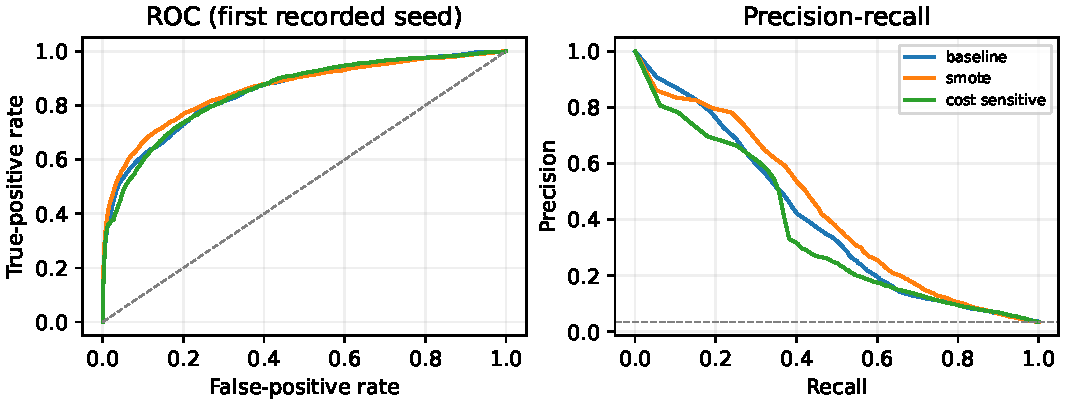
\includegraphics[width=0.95\linewidth]{figures/comparison.pdf}
\caption{Final-test ROC and precision--recall curves for seed 42. The horizontal PR reference is test fraud prevalence.}
\end{figure}

\begin{table}[ht]
\centering\small
\caption{Seed-42 operational counts and timing. Inference excludes preprocessing and HTTP overhead.}
\begin{tabular}{lrrrrr}
\toprule Method & $\tau$ & FP & FN & Train (s) & Infer (s) \\
\midrule
Baseline ANN & 0.13 & 1512 & 1881 & 134.1 & 0.015 \\
SMOTENC + ANN & 0.59 & 1760 & 1688 & 161.2 & 0.015 \\
Weighted ANN & 0.81 & 2028 & 1932 & 122.1 & 0.018 \\
\bottomrule
\end{tabular}
\end{table}

\subsection{Development and Threshold Analysis}
Baseline ANN development AP is 0.2463 $\pm$ 0.0046 across 3 seeds. SMOTENC + ANN development AP is 0.2656 $\pm$ 0.0247 across 3 seeds. Weighted ANN development AP is 0.2186 $\pm$ 0.0020 across 3 seeds.
These smaller runs share one sample/holdout; their variation is distinct from full-data variation. Lower cutoffs can recover missed fraud while increasing legitimate alerts. Validation-F1 selection is a comparison rule, not a monetary-cost optimum: operational costs and review capacity were not supplied.

\section{Comparison with Existing Work}
The literature provides context rather than a numerical leaderboard. Review coverage, different datasets, feature spaces, resampling practices, models, and unmatched splits preclude score ranking \cite{cheah2023smotegan,hayat2025leakage,darwish2025abc,habibpour2023uncertainty}. External superiority would require faithful reimplementation under a common untouched test set and equal tuning budgets. This study establishes an internal controlled comparison only.

Two supplied notebooks inform EDA and future feature engineering. The XGB reference combines train/test covariates for aggregates and applies label-informed UID post-processing. These are competition-specific operations, not this inductive protocol. The EDA reference overwrites TimeSeriesSplit with KFold; sorting alone does not create forward-time validation. Their leaderboard claims are not adopted as our results.

\section{Discussion and Limitations}
Results are bounded by the feature subset, network family, training budget, and temporal window. Chronological holdout does not reproduce evolving labels, infrastructure, customer populations, or adversaries. Exact duplicate removal is weaker than entity-disjoint evaluation.

Weighting and resampling can alter score calibration. Sigmoid percentages remain model scores until natural-prevalence calibration is assessed. Full-data repeated seeds strengthen reproducibility but do not establish generalization across temporal windows. IID intervals require caution under correlated transactions.

Integrated gradients use 64 steps on the model logit relative to an all-zero encoded baseline. That baseline can be outside the data manifold. Contributions indicate model sensitivity, not causal evidence or calibrated probability decomposition.

Dense-matrix guards do not include all raw CSV parsing memory. Timings depend on hardware and realized early stopping. Serialized preprocessors must be trusted. Remote hosting needs private authentication, explicit origins, durable artifacts, and backups. Deployment configurations separate Vercel frontend hosting from persistent Python API/worker processes; no public deployment is inferred from local success.

\section{Conclusion}
Three distinct ANN imbalance strategies are implemented within a reproducible end-to-end laboratory. Shared temporal holdouts, training-only transformations, validation selection, and canonical artifacts make measured comparisons auditable. Ranking and alert trade-offs are reported with scope and uncertainty explicit. The application supports research and inspection without claiming production financial validity.

\section{Future Scope}
Priorities are repeated temporal windows, entity-disjoint tests, separate calibration, cost-aware cutoffs, conventional baselines under equal budgets, and training-only or past-only group features. Uncertainty estimation, drift monitoring, and shared database/object storage could improve robustness. Extensions must preserve the final-test boundary.

\clearpage
\bibliographystyle{IEEEtran}
\bibliography{references}
\end{document}
